\documentclass[11pt,a4paper,fontset=none]{ctexart}
\usepackage[margin=1.1cm]{geometry}
\usepackage{xcolor}
\usepackage{tabularx}
\usepackage{enumitem}
\usepackage{titlesec}
\usepackage{array}
\usepackage{setspace}
\usepackage{ragged2e}
\usepackage{graphicx}

\setCJKmainfont[Path=C:/Windows/Fonts/,BoldFont=msyhbd.ttc]{msyh.ttc}
\setCJKsansfont[Path=C:/Windows/Fonts/,BoldFont=msyhbd.ttc]{msyh.ttc}
\setCJKmonofont[Path=C:/Windows/Fonts/]{simsun.ttc}

\pagestyle{empty}
\setlength{\parindent}{0pt}
\setlength{\parskip}{0pt}
\setstretch{1.03}
\definecolor{mainblue}{HTML}{2F5597}
\definecolor{resumeTeal}{HTML}{436A78}
\definecolor{resumeGold}{HTML}{C5A46A}
\definecolor{lightgray}{HTML}{F4F6FA}
\definecolor{textgray}{HTML}{333333}
\setlist[itemize]{leftmargin=1.05em,itemsep=0em,topsep=0.04em,parsep=0em}
\newcommand{\sectionTag}[1]{%
  \noindent\colorbox{resumeTeal}{\makebox[2.9cm][l]{\hspace{0.45em}\color{white}#1}}%
  \hspace{0.1cm}{\color{resumeTeal}\rule[0.55ex]{\dimexpr\linewidth-3.35cm\relax}{0.35pt}}%
}
\titleformat{\section}{\large\bfseries}{}{0em}{\sectionTag}
\titlespacing*{\section}{0pt}{0.5em}{0.25em}
\renewcommand\labelitemi{\textcolor{mainblue}{\small$\bullet$}}

\newcommand{\resumeHeader}[5]{
  \noindent
  \begin{minipage}[t]{0.72\linewidth}
    {\zihao{1}\color{resumeTeal}\bfseries 个人简历}
    {\color{resumeTeal}\hspace{0.35em}\rule[-0.35em]{0.8pt}{2.4em}\hspace{0.7em}}
    \begin{minipage}[b]{0.38\linewidth}
      {\small 细心从每一个细节开始}\par
      {\zihao{4}\color{resumeTeal}Personal resume}
    \end{minipage}
  \end{minipage}
  \par
  \vspace{0.35em}
  {\color{resumeTeal}\rule{0.61\linewidth}{6pt}}{\color{resumeGold}\rule{0.39\linewidth}{6pt}}\par
  \vspace{0.25em}
}

\newcommand{\entry}[4]{
  \vspace{0.15em}
  \noindent
  \makebox[3.8cm][l]{\bfseries\color{mainblue}#1}%
  \makebox[10.1cm][c]{\bfseries #2}%
  \makebox[4.6cm][r]{\bfseries #3}\par
  \if\relax\detokenize{#4}\relax\else {\color{textgray}#4}\fi
}

\newcommand{\projectTitle}[4]{
  \vspace{0.2em}
  \noindent
  \makebox[4.9cm][l]{\bfseries\color{mainblue}#1}%
  \makebox[8.8cm][c]{\bfseries #2}%
  \makebox[4.8cm][r]{\bfseries #3}\par
  {\color{textgray}#4}
}

\begin{document}
\color{textgray}
\resumeHeader{吴亮希}{个人简历 \quad Personal Resume}{21岁 / 女 / 汉族 / 汕头}{19865923115}{202200202067@stumail.sztu.edu.cn}

\section{基本信息}
\begin{minipage}[t]{0.74\linewidth}
  \vspace{0pt}
  \begin{tabularx}{\linewidth}{@{}p{1.85cm}X p{1.85cm}X@{}}
  姓\quad 名： & 吴亮希 & 年\quad 龄： & 21岁 \\
  性\quad 别： & 女 & 身高体重： & 165cm/51kg \\
  民\quad 族： & 汉 & 籍\quad 贯： & 汕头 \\
  政治面貌： & 共青团员 & 电\quad 话： & 19865923115 \\
  邮\quad 箱： & \multicolumn{3}{l}{202200202067@stumail.sztu.edu.cn} \\
  GitHub： & \multicolumn{3}{l}{github.com/wanlixing-dream} \\
  \end{tabularx}
\end{minipage}
\hfill
\begin{minipage}[t]{0.20\linewidth}
  \vspace{-0.45cm}
  \raggedleft
  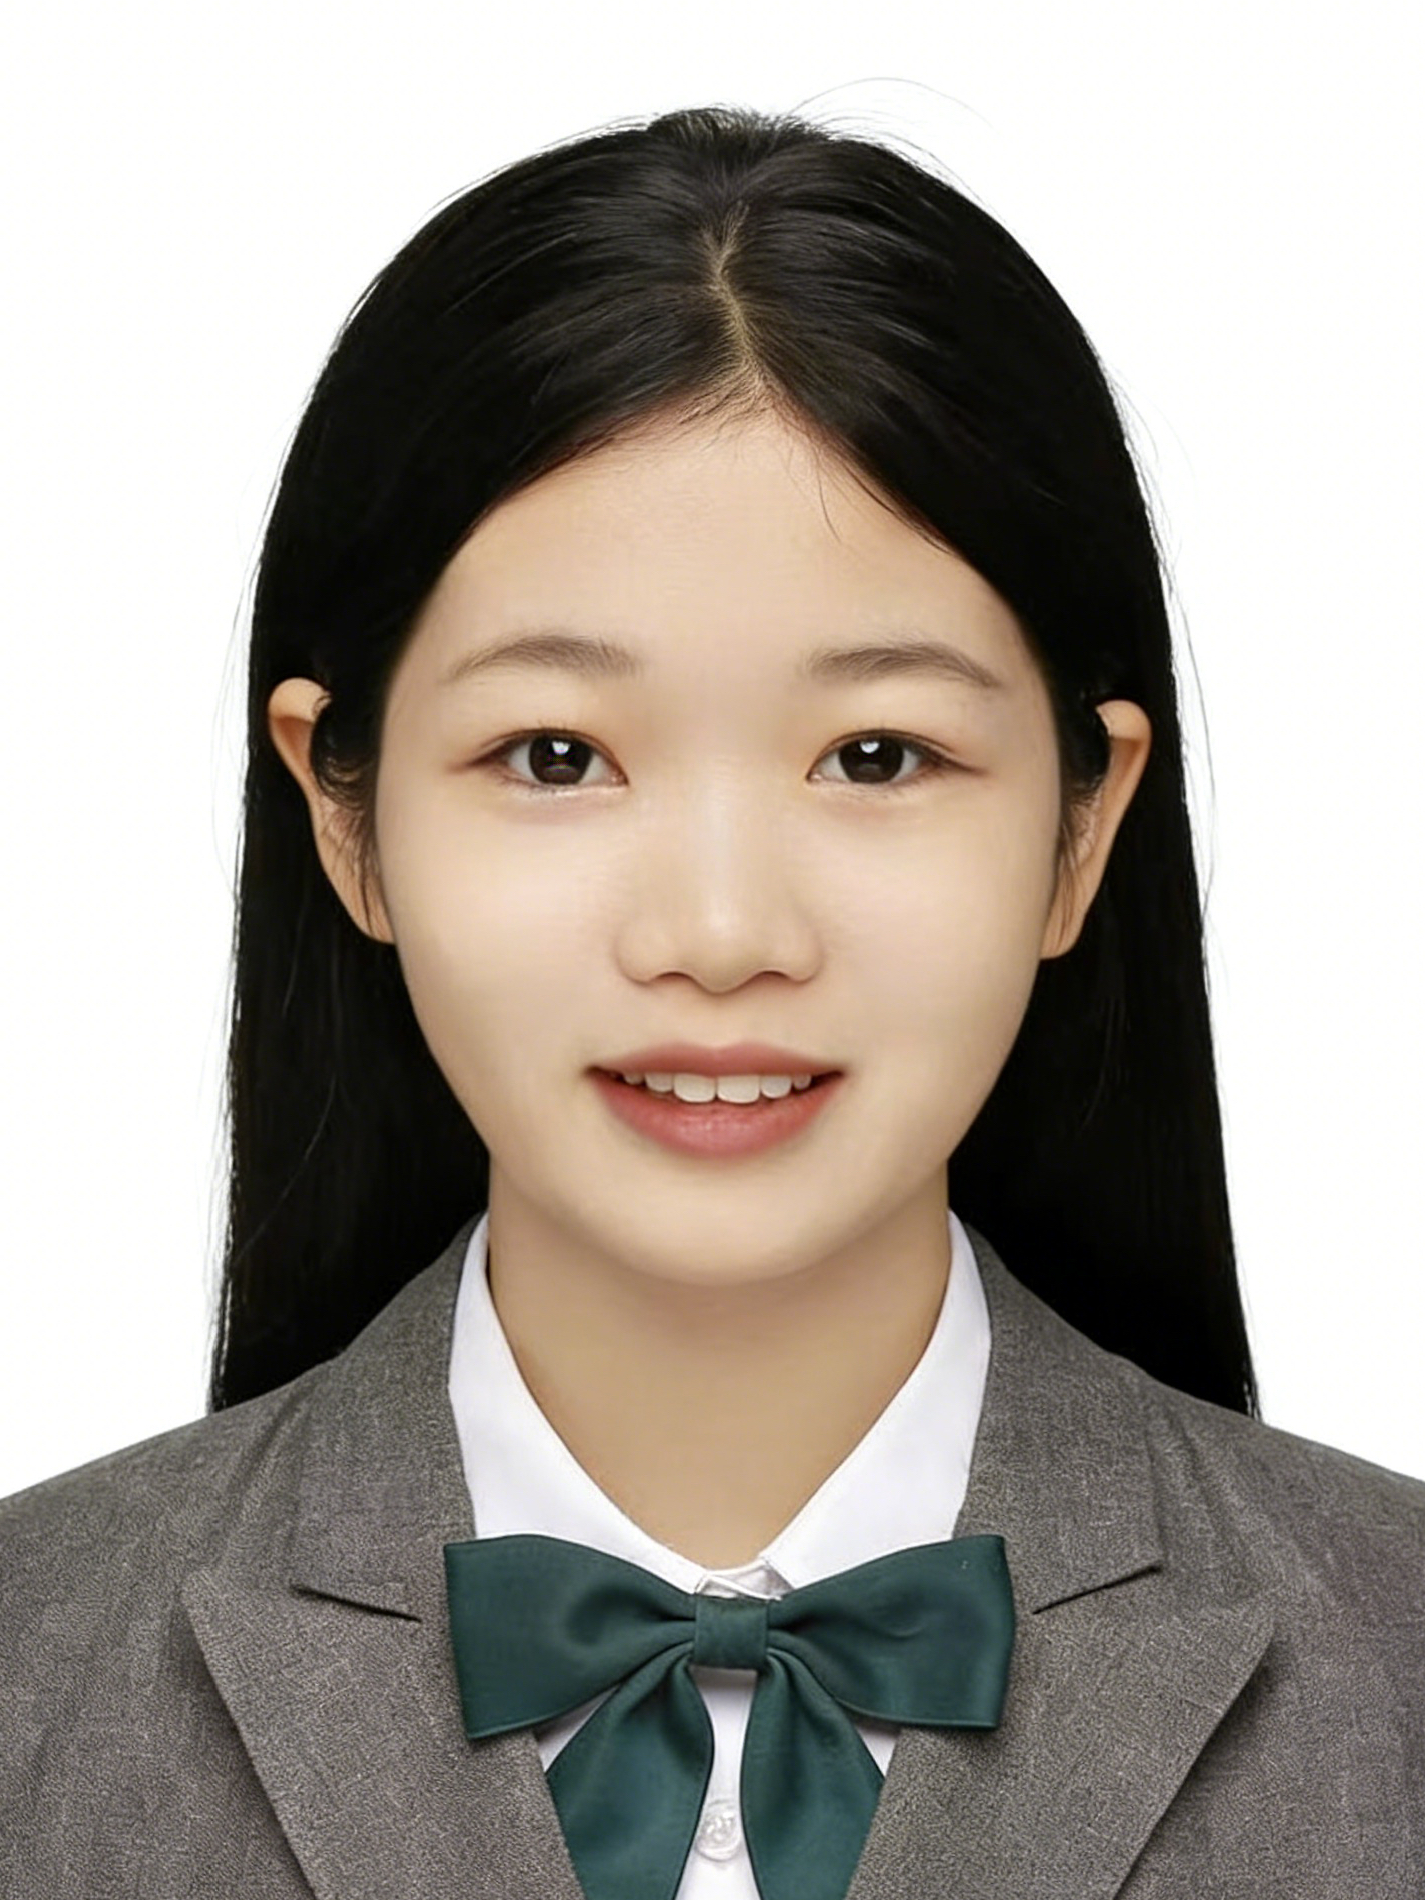
\includegraphics[width=2.55cm,height=3.35cm,keepaspectratio]{photo.jpg}
\end{minipage}

\section{教育背景}
\entry{2022-09 至今}{深圳技术大学}{计算机科学与技术（本科）}{}
\begin{itemize}
  \item 核心课程：数据库系统、软件工程、计算机网络、数据结构与算法、操作系统、人工智能导论、大数据原理、深度学习。
  \item 入选伦琴人工智能实验班（百度联合培养，前 10\%），计算机生物学实验室算法组核心成员。
\end{itemize}

\section{实习经验}
\projectTitle{2026-01 至 2026-05}{百思特管理咨询有限公司}{AI 工程师实习生}{项目内容：}
\begin{itemize}
  \item 参与 BestCowork 企业级 AI 协作平台研发，围绕数字员工、技能市场、知识库绑定、沙箱执行和 AI 工作流等功能推进可复用 Agent 模块落地。
  \item 参与 Agent EngineRouter、团队注册表、委托工具、会话状态和工具权限等核心模块联调，熟悉 LLM、知识库、工具/API 与业务系统之间的任务编排和上下文传递。
  \item 基于 Electron+React+TypeScript 参与桌面端产品建设，配合客户端状态、IPC 通信、接口联调、日志排查、测试验证和版本迭代，理解 AI 产品从原型验证到业务交付的流程。
  \item 技术栈：TypeScript、React、Electron、Node.js、SQLite、LLM API、Agent Engine、MCP/工具调用、Git。
\end{itemize}
项目职责：
\begin{itemize}
  \item 参与单 Agent/团队模式执行链路验证，围绕任务委托、并行委托、子会话创建、超时处理、错误返回和状态同步进行问题定位与效果复盘。
  \item 参与技能服务启动、运行时 PATH 处理、工具调用、权限请求、健康检查、引擎降级和异常恢复等能力验证，沉淀测试用例、使用说明和问题排查记录。
  \item 与产品、前端和业务团队协作推进交付，参与需求理解、问题定位、设计说明和使用文档整理，关注 Agent 在真实业务流程、客户端交互和任务自动化中的可用性。
\end{itemize}

\section{项目经验}
\projectTitle{2024-10 至 2024-12}{个性化 AI 学习与 RAG 智能体系统}{负责人}{项目内容：}
\begin{itemize}
  \item 从 0 到 1 搭建个人开源 Agent 项目，实现 create/add/vibe/summary 等意图识别、任务路由、活跃会话状态管理和多轮互动，可作为 GitHub 项目展开讲解。
  \item 设计长期记忆与上下文数据持久化方案，使用 JSONL 分片、ChromaDB 向量库、BM25 倒排索引和 TF-IDF/实体/重要性/时效融合实现 RAG 混合检索。
  \item 封装 FastAPI REST API 与 MCP Tools，提供学习领域、知识笔记、进度摘要、记忆搜索、薄弱概念、掌握度更新、链路追踪和执行评估等接口。
  \item 技术栈：Python、FastAPI、ChromaDB、BM25、RAG、MCP、Prompt Engineering、React、TypeScript、Git。
\end{itemize}
项目职责：
\begin{itemize}
  \item 负责后端系统分层设计，将能力拆分为 API 层、核心服务层、记忆存储层、RAG 检索层、MCP 工具层、链路追踪和评估模块，便于智能应用能力复用。
  \item 设计 Prompt 与工具调用流程，支持知识添加、摘要生成、记忆搜索、薄弱点查询和掌握度更新，形成可复用的 Agent 问答和知识管理能力。
  \item 设计 TraceRecorder 与 AgentEvaluator，记录 intent、memory/RAG 检索、LLM 调用、工具调用、错误恢复等步骤，并用工具成功率、记忆使用、输出格式等维度评估执行质量。
\end{itemize}

\newpage
\vspace*{0.65cm}
\projectTitle{2026-05 至 2026-05}{WanliDeal 端到端 AI 数据处理产品}{负责人}{项目内容：}
\begin{itemize}
  \item 从 0 到 1 搭建前后端打通的优惠信息验证助手，覆盖文本提交、URL 提取、字段抽取、时效校验、结构化存储、API 查询和前端展示。
  \item 基于 LiteLLM 调用大模型并设计严格 JSON 输出 Prompt，将微信群/手动录入的非结构化信息解析为商品、链接、价格、平台、步骤和有效期等字段。
  \item 提供一键启动脚本，自动检查环境、创建虚拟环境、安装前后端依赖并启动 FastAPI 与 Vue 前端，便于端到端演示和迭代。
  \item 技术栈：Python、FastAPI、SQLAlchemy、SQLite、LiteLLM、Pydantic、pytest、Vue 3、TypeScript、Git。
\end{itemize}
项目职责：
\begin{itemize}
  \item 负责从原始消息到结构化卡片的处理链路设计，将流程拆分为 Extractor、Validator、Formatter、Pipeline、DB 和 API 层，便于快速调整产品规则。
  \item 编写 URL 正则提取、LLM JSON 解析、字段映射、原始消息保存、结构化入库、条件筛选和分页查询逻辑，覆盖数据采集、清洗、字段整理与管理。
  \item 编写 API、抽取器、处理流水线、格式化器和校验器测试用例，覆盖健康检查、批量提交、LLM 返回解析失败、时效校验和数据格式转换等场景。
\end{itemize}

\section{技能特长}
\begin{itemize}
  \item 编程语言：熟练 Python，掌握 TypeScript/JavaScript，掌握 Java 基础，了解 C/C++；具备数据结构与算法基础，蓝桥杯 Python B 组省级二等奖。
  \item 编程与后端：熟练 Python，实践 FastAPI、Pydantic、SQLAlchemy、SQLite、REST API、参数校验、异常处理、分页查询、JSON 序列化和 pytest 测试。
  \item 客户端与前端：实践 Electron、React、Vue 3、TypeScript、IPC 通信、状态管理、前端数据展示和桌面端调试，理解客户端复杂模块交付。
  \item AI Native 与智能体：熟悉 Prompt Engineering、RAG、ChromaDB、BM25、TF-IDF、MCP Tools、意图识别、多轮会话状态、工具调用和智能问答接口封装。
  \item 后端与端到端：实践 Python、FastAPI、Pydantic、SQLAlchemy、SQLite、REST API、参数校验、异常处理、分页查询、JSON 序列化和 pytest 测试。
  \item Agent 工作流：长期使用 Cursor/Trae 等 AI 编程工具辅助需求拆解、代码生成、测试排错和文档整理，关注“为什么做”、功能取舍和可交付闭环。
  \item 产品理解：关注 Agent 产品从需求判断、交互设计、功能取舍到测试验证的完整闭环，能够将知识库和大模型能力落到具体业务流程。
  \item 语言：CET-6，可熟练读写与沟通。
\end{itemize}

\section{荣誉证书}
\begin{itemize}
  \item 2025年5月26号 \quad 蓝桥杯全国软件和信息技术专业人才大赛 Python 程序设计 B 组 \quad 省级二等奖。
  \item 2025年12月30日 \quad 科创之星三等奖、学习之星二等奖、文体之星三等奖 \quad 校级。
  \item 2024年四月 \quad 优秀共青团员 \quad 校级。
\end{itemize}

\section{自我评价}
本人计算机专业基础扎实，系统学习数据库、操作系统、计算机网络、数据结构与算法、人工智能、深度学习等课程。具备企业级 AI 协作平台实习经验，以及在校期间完成的 0→1 RAG 智能体系统和端到端 AI 数据处理产品经验，熟悉 Electron/React、Vue、TypeScript、Python、FastAPI、大模型 API、Prompt Engineering、RAG、MCP 工具调用、测试验证和可视化展示。习惯借助 Agent 工具拆解需求、生成方案、实现功能和排查问题，关注 AI 产品从需求判断、方案设计、功能实现到验证迭代的完整链路，愿意参与产品定义并主动判断功能价值。

\section{兴趣爱好}
编程、跳舞、弹吉他、写书法。

\end{document}
